%!TEX root = presentazionelancia.tex
\section{Architecture}
\begin{frame}[t]
\frametitle{Architecture}
    \onslide<1>Before Tao
    \onslide<1>\begin{center}
    	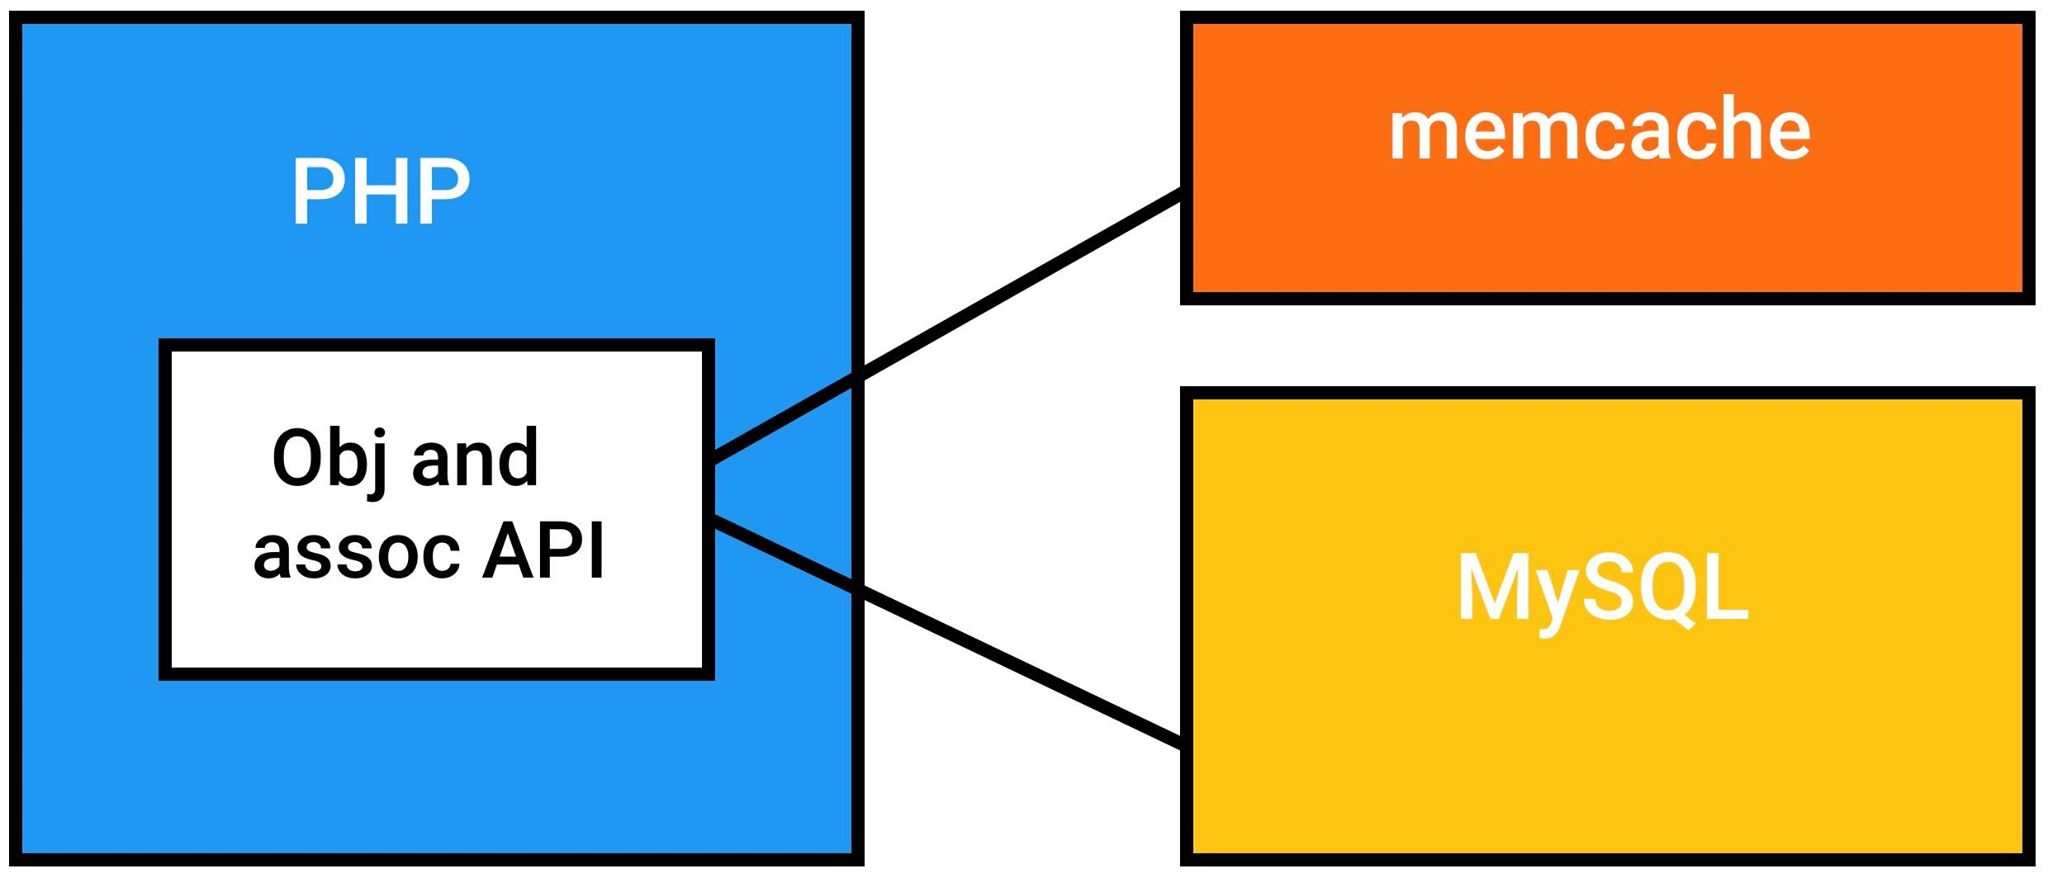
\includegraphics[width=0.4\textwidth]{figs/before_tao.jpg}
    \end{center}
	\onslide<2>After Tao
	\onslide<2>\begin{center}
    	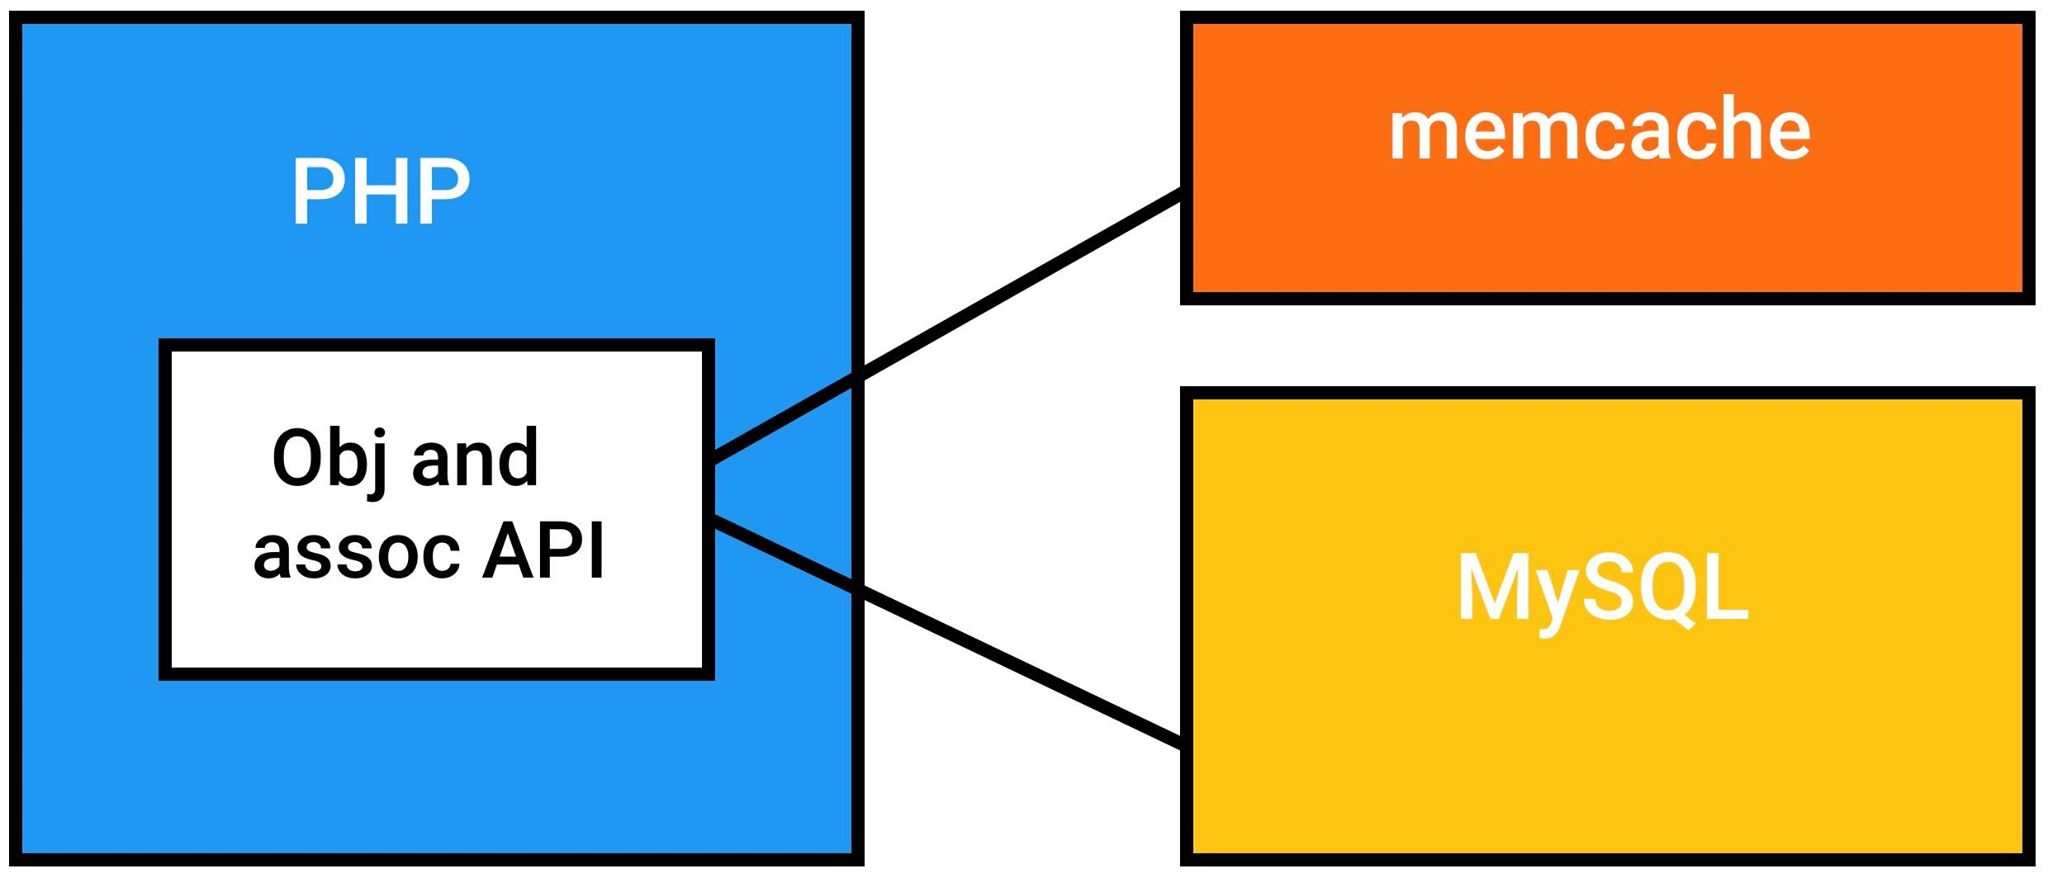
\includegraphics[width=0.4\textwidth]{figs/before_tao.jpg}
    \end{center}
\end{frame}

\begin{frame}[fragile]
\frametitle{Storage Layer}
\begin{itemize}
	\item Object and Associations are stored in MySql (before \& with TAO)	
	\item TAO API is mapped to a small set of SQL queries
	\item A single MySql server can't handle TAO volumes of data
	\begin{itemize}
		\item We divide data into logical \emph{shards}
		\item \emph{shards} are mapped to db 
		\item different servers are responsible for multiple shards
		\item mapping is adjusted for load balancing
	\end{itemize}
	\item Object are bounded to a \emph{shard} for their entire lifetime
	\item Associations are stored in the \emph{shard} of its \verb!id1!
\end{itemize}




    


\end{frame}
